\documentclass[11pt]{article}

\usepackage{geometry}
\geometry{a4paper, portrait, margin=2cm}

\usepackage{helvet}
\renewcommand{\familydefault}{\sfdefault}

\usepackage{setspace}
\usepackage{indentfirst}

\usepackage{parskip}
\usepackage{lineno}
\usepackage{graphicx}
\usepackage{natbib}
\usepackage[T1]{fontenc}

%opening

\begin{document}

	\begin{titlepage}
		
		\centering
			
		\vspace*{3cm}
		\LARGE
		MSc CMEE Project Proposal
		
		\vspace*{7cm}
		\Huge
		\textbf{Developing NFTs for sparrows}\\
		
		\vspace{2cm}
		\LARGE
		
		\vfill
		
		\begin{flushleft}
			
		\large
		
		\textbf{Student:}\\
		An Nguyen\\
		an.nguyen21@imperial.ac.uk\\
		
		\vspace{1cm}
		
		\textbf{Supervisor:}\\
		Dr Julia Schroeder\\
		julia.schroeder@imperial.ac.uk\\
	
		\vspace{2cm}
		\end{flushleft}

	\end{titlepage}
	
	\linenumbers
	\onehalfspacing
\textbf{Keywords:} Machine Learning; Blockchain; Cryptocurrency

\section*{Introduction}
		
		Non-fungible token (NFT) represents data stored on the blockchain, a type of of digital ledger. As NFT is non-fungible, it is unique, non-interchangeable, and irreplaceable \citep{city27164} \citep{math10030335}. Each token is one of a kind, making NFT particularly suitable for certifying and tracking ownership of unique assets \citep{city27164}. The initial NFTs were built on the Ethereum blockchain but they have now expanded to other blockchains \citep{city27164} \citep{10.1007/978-981-16-3961-6_34}. A smart contract stores the information needed to carry out an NFT transfer on the blockchain \citep{10.1007/978-981-16-3961-6_34}. 
		
		\hspace{4ex} The existing Lundy House sparrow database includes various entries about the sparrows; however, there is no unique artwork associated with any of the sparrows. To automate the process of art creation, the machine learning model called generative adversarial network (GAN) will be used \citep{DBLP:journals/corr/abs-2112-10577}. GAN is a deep learning framework involving two neural network-based models known as generators and discriminators \citep{AGGARWAL2021100004}. The generator network synthesizes new candidates which will then be evaluated by the discriminator; the discriminator examines whether the data are from the real distribution or generated by the generator \citep{AGGARWAL2021100004}. The two networks are trained simultaneously, the goal is for the generator to fool the discriminator into thinking that candidates are not synthesized about half of the time \citep{DBLP:journals/corr/abs-2112-10577} \citep{AGGARWAL2021100004}. GAN will be used to superimpose different art styles onto the sparrow photos \citep{DBLP:journals/corr/abs-1711-06454}. 
	
	\section*{Methods}
		Example images for style transfer will be obtained from the NFT art collection. CycleGAN, an image-to-image translation model, will be tested first to see if the art style is successfully transferred to the target images. The model will be Python-based. NFT smart contracts will be written in JavaSript and deployed to the Stellar blockchain.
		
	\section*{Project Aims}
		\begin{itemize}
			\item Build a model which can change the style of the target image based on another image.
			\item Deploy NFT smart contracts on the blockchain.
		\end{itemize}
		
	\section*{Timeline}
		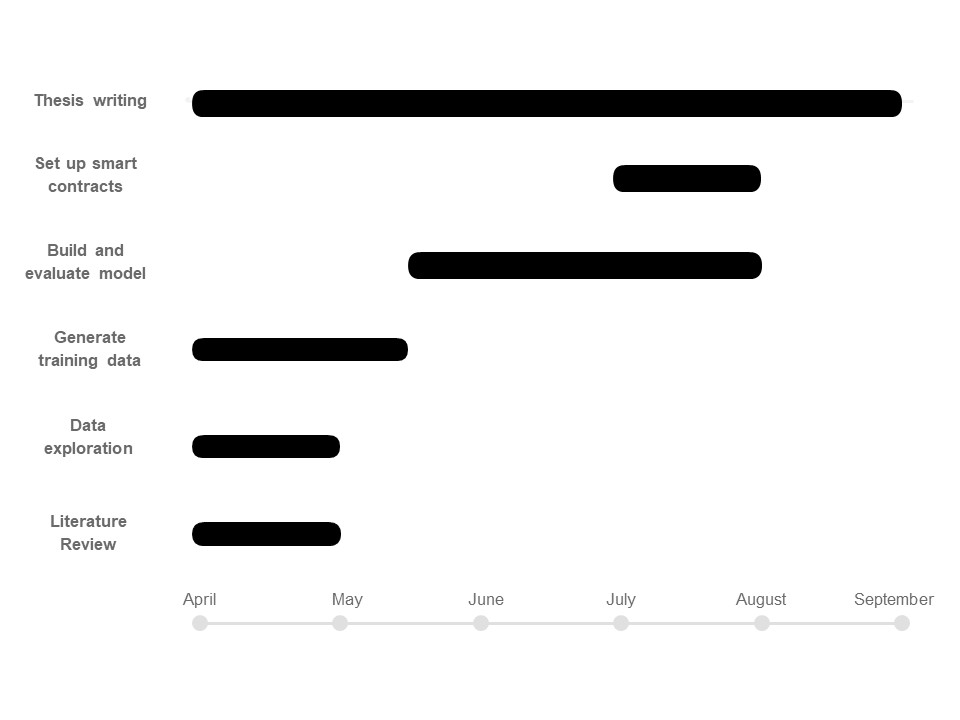
\includegraphics[width = \textwidth]{gantt.jpg}
		
	\bibliographystyle{abbrvnat}
	\bibliography{propsal}
\end{document}
